\subsection{Approximation of a porous medium} \label{sec:approx-porous-medium}

	\begin{figure}[H]
		\centering
		\begin{subfigure}{0.55\textwidth}
			\centering
			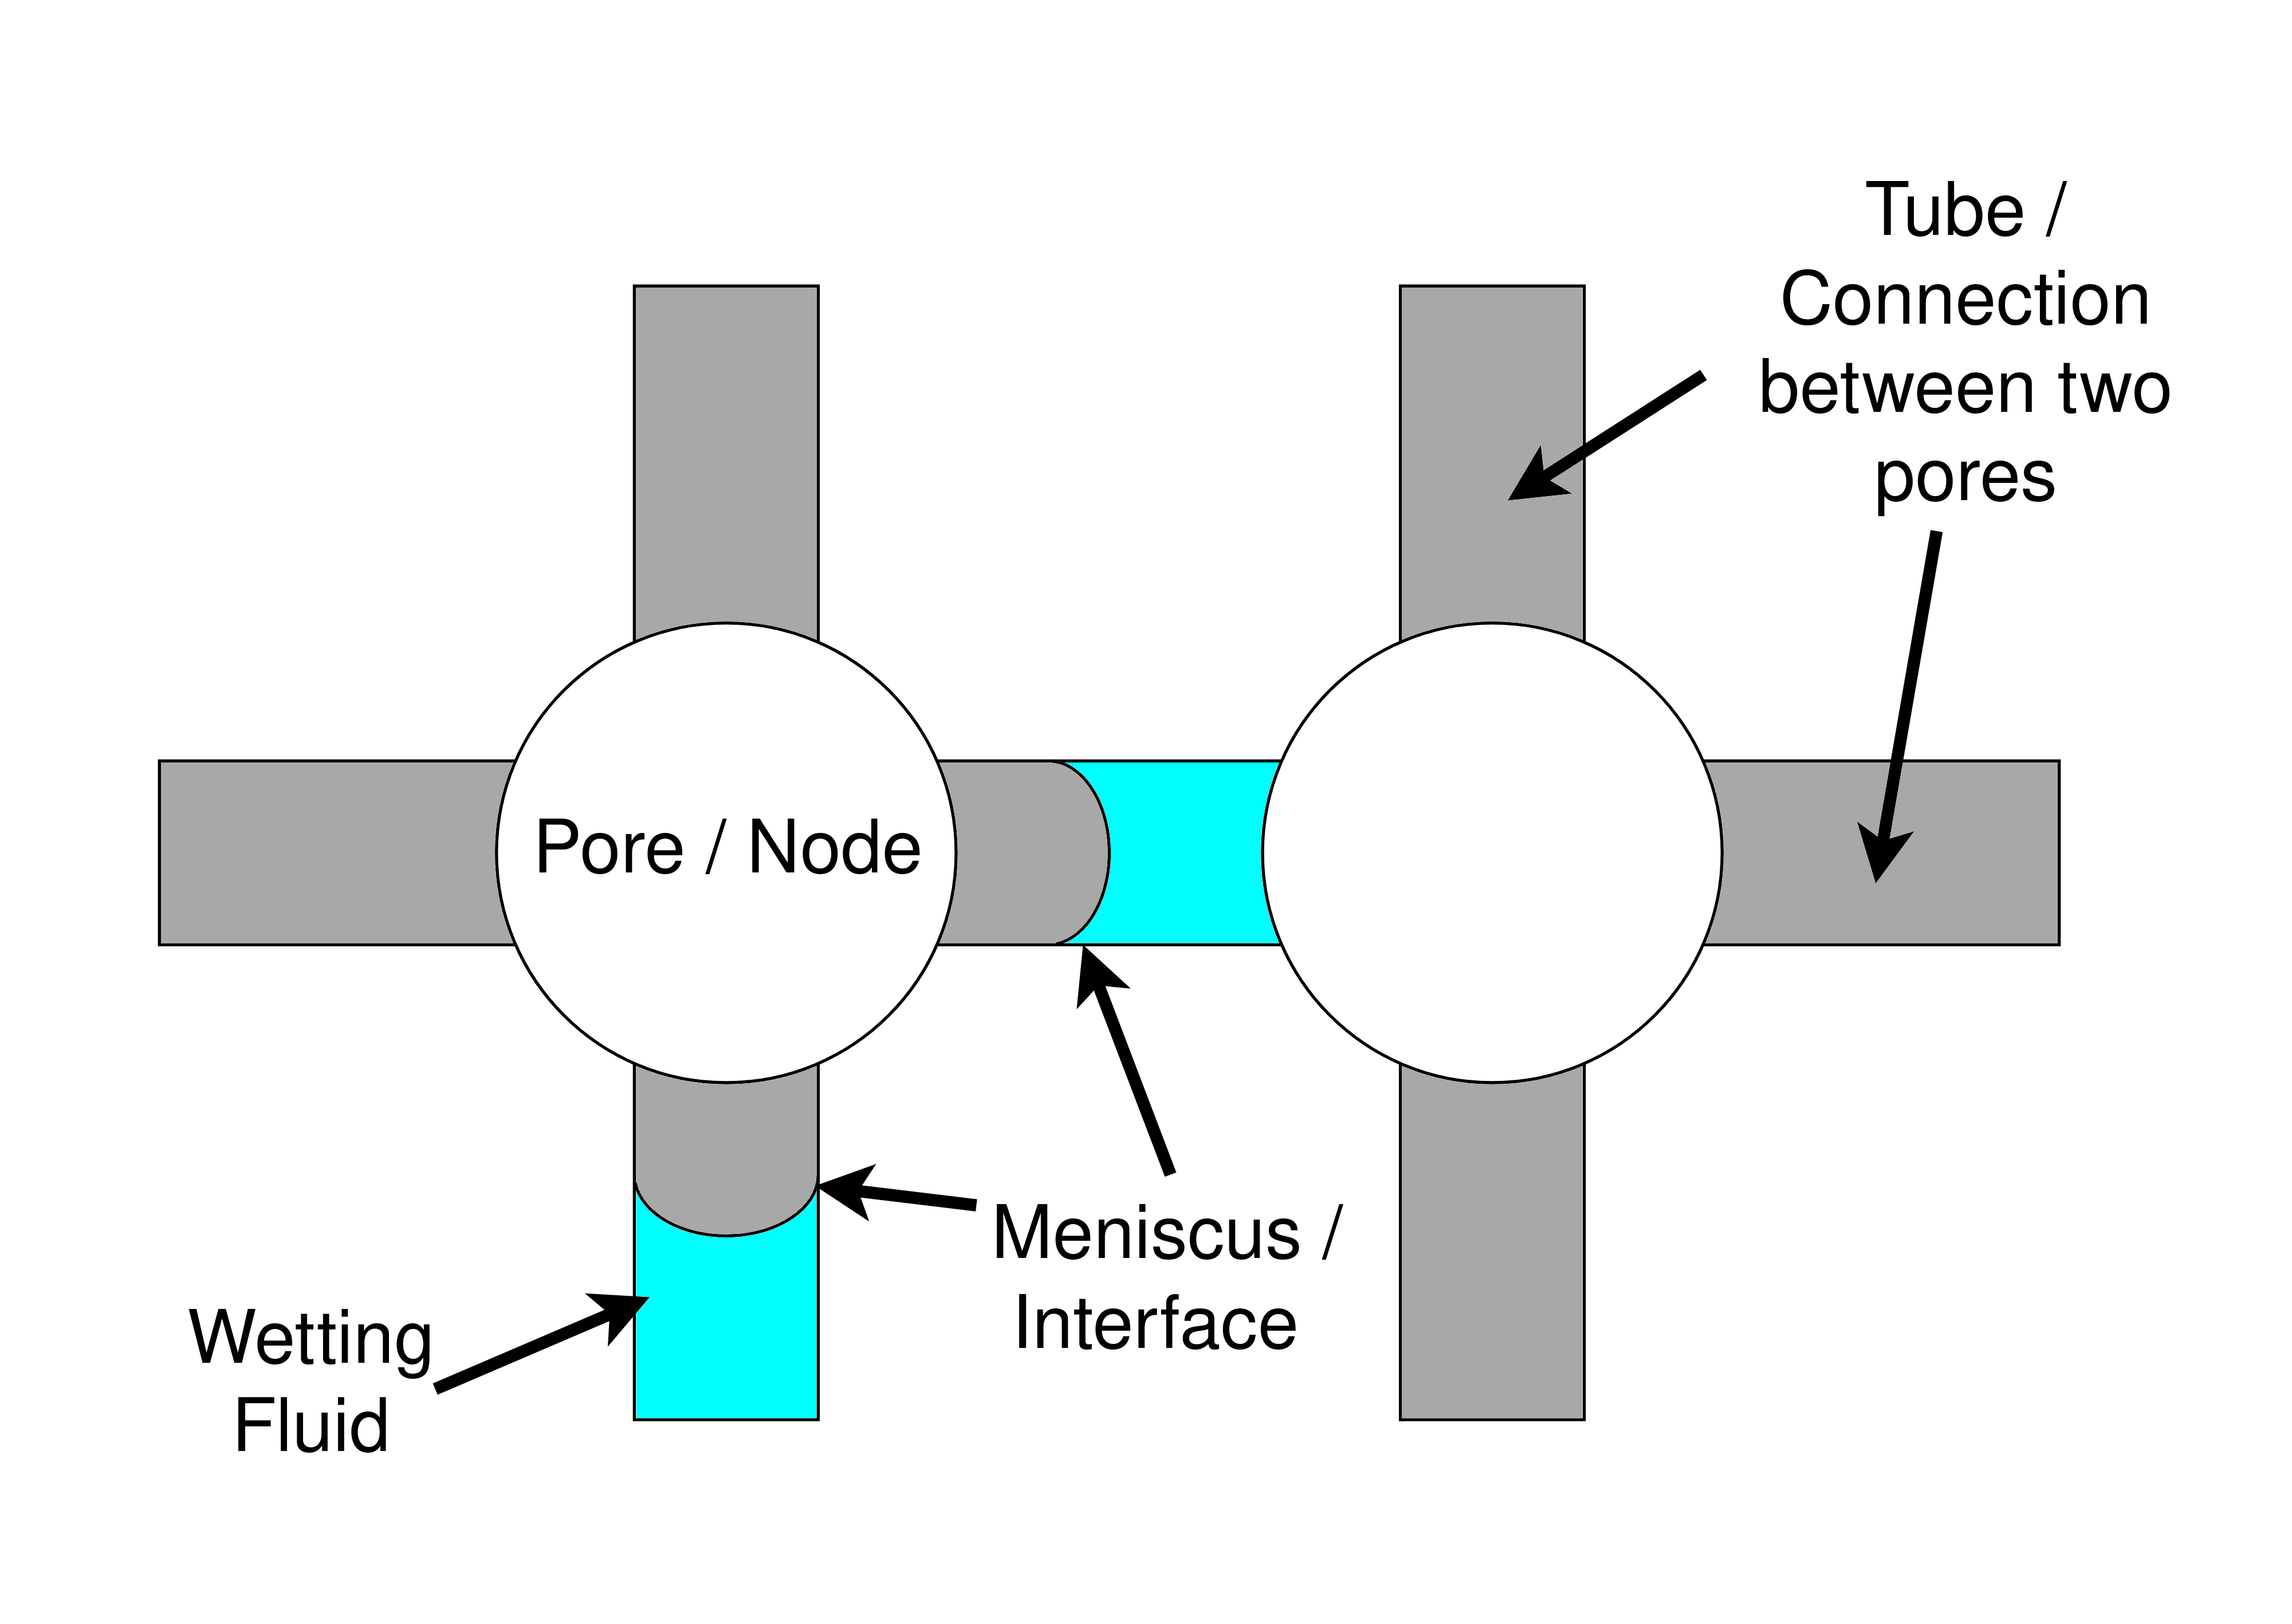
\includegraphics[width=\textwidth]{fig_descp-of-model}
			\caption{Pore as node, and capillary as tube}
			\label{fig:descp-of-model}
		\end{subfigure}
		\begin{subfigure}{0.4\textwidth}
			\centering
			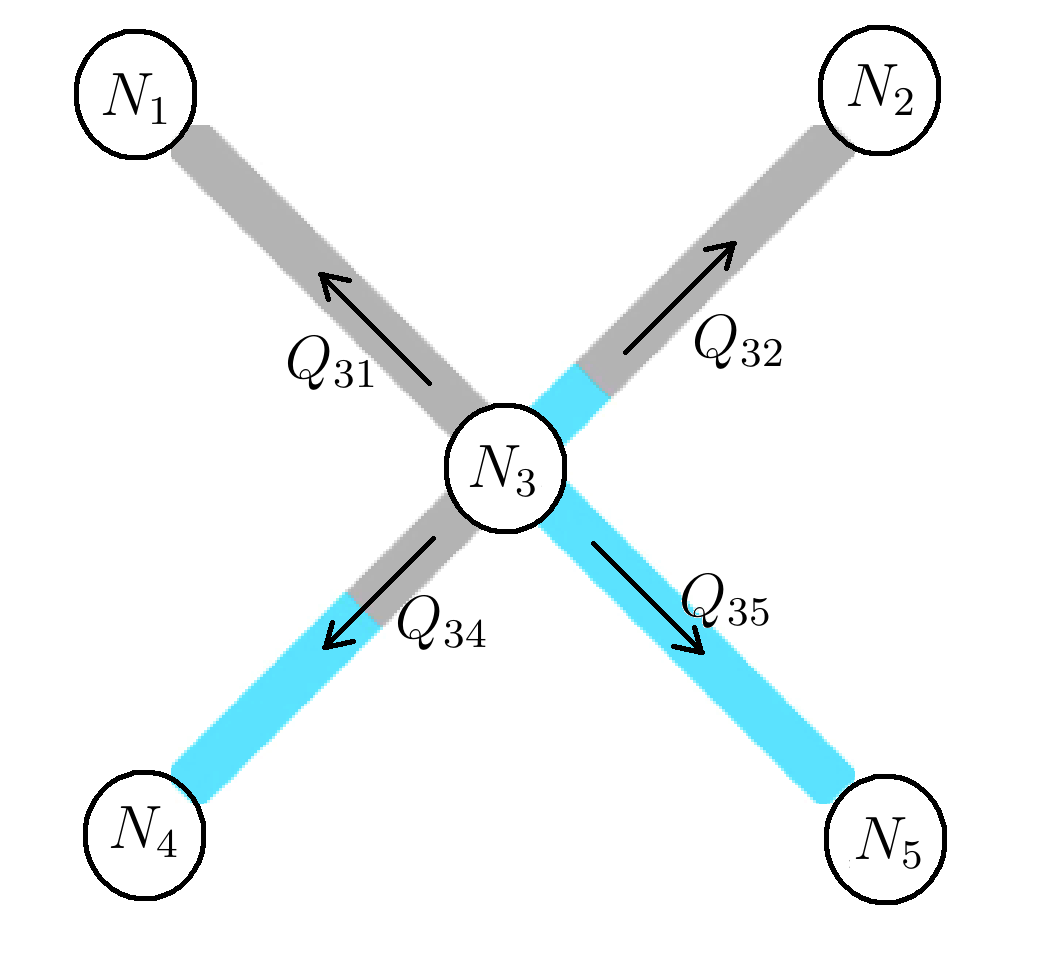
\includegraphics[width=\textwidth]{fig_simple-5-nodes}
			\caption{Flow rates in tubes connected to a node.}
			\label{fig:simple-5-nodes}
		\end{subfigure}
		\caption{Network model of porous medium.}
	\end{figure}
	
	A porous medium consists of pores, which are connected by capillaries. The pores are represented by nodes, while the capillaries are represented by tubes, as shown in figure \ref{fig:descp-of-model}. Our model is two-dimensional. Each node is connected to 4 other nodes through tubes, shown in figure \ref{fig:simple-5-nodes}. They may be connected to less than 4 nodes, when they are located on the boundaries. The color cyan denotes wetting fluid, while the color gray denotes non-wetting fluid.
		
	Gravity is ignored. The fluids are not compressible. The volume of the node is not taken into consideration and is assumed to be zero. All tubes are of equal length and cylindrical. The tubes can have different radii. The capillary pressure is zero inside the node. A tube can have a maximum of 2 menisci. The novelity of our model is that during flow, when both cyan and gray fluid enters one node, then the fluids are distributed such that the cyan fluid is distributed first to the thinner tubes. If a tube has more than two meniscus, then there are combined together such that the center of mass of each fluid remains the same.
	
	Note that the assumption of zero volume of node would not change the mixing of different fluids. Let us assume that a node with non-zero volume is filled with gray fluid is invaded by cyan fluid. Since the cyan fluid is distributed first, it immediately reaches the ends of the other tubes connected to the node. The assumption of zero volume of node only affects how the saturation is calculated, never the less it was assumed to be zero to keep the calculations simple.

\subsection{Set of linear equations for a node} \label{sec:linear-equ}
	
	Let the flow rate in a tube be given by:
	\begin{equation}  \label{eq:flow-rate-simple-coeff}
		Q_{ij} = A_{ij}\Delta P_{ij} + B_{ij}
	\end{equation}
	
	Here, $Q_{ij}$ is the flow rate form node $N_i$ to node $N_j$. $A_{ij}$ and $B_{ij}$ are real constants. Here $\Delta P_{ij} = P_i - P_j$, where $N_i$ is kept at a pressure of $P_i$ and $N_j$ at a pressure of $P_j$. The detailed form is given by equation \ref{eq:main-flow-rate-with-s}
	
	During simulation, we produce a set of linear equations. We iterate through each node, write equations of flow rates for each tube connected to the node, and equate the sum to zero. For each node, we get one row of the linear equation augmented. For figure \ref{fig:simple-5-nodes}:
	
	\begin{equation}
		Q_{3j} = A_{3j}\Delta P_{3j} + B_{3j}
	\end{equation}

	Due to the conservation of volume, we have:
	\begin{equation}
		\sum_{k} Q_{3k} = 0
	\end{equation}
	
	Where $k = {1, 2, 4, 5}$.
	
	Note that all $Q$'s point outward. The $Q$'s will have different signs in order to preserve the law of conservation of volume. For fluid flowing out of $N_3$, we will have $Q_{3j} > 0$, while for fluid flowing into $N_3$, we will have $Q_{3j} < 0$.
	
	Let us assume that the pressures at all nodes are known, except $N_3$. Then, the set of linear equations would look like:
	
	\begin{equation} \label{eq:matrix-open-sys-5-nodes}
		\begin{pmatrix}
			1 & 0 & 0 & 0 & 0 & P_{1}\\
			0 & 1 & 0 & 0 & 0 & P_{2}\\
			-A_{31} & -A_{32} & (A_{31} + ... + A_{35}) & -A_{34} & -A_{35} & -(B_{31} + ... + B_{35})\\
			0 & 0 & 0 & 1 & 0 & P_{4}\\
			0 & 0 & 0 & 0 & 1 & P_{5}
		\end{pmatrix}
	\end{equation}

\subsection{Average Capillary Pressure}
	The average capillary pressure in a region is defined as:
	\begin{equation} \label{eq:average-capillary-pressure}
		P_c = \frac{\sum \frac{2 \sigma}{r_i} s_i \pi r_i^2}{\sum s_i \pi r_i^2}
	\end{equation}
	
	Here $\sigma$ is the coefficient of surface tension. And $r_i$ is the radius of the tube.
	
	\begin{equation} \label{eq:average-capillary-pressure-sign}
		s_i = 
		\begin{dcases}
			0,&\text{even number of meniscus in the tube}\\
			1,&\text{odd number of meniscus in the tube}\\
		\end{dcases}
	\end{equation}
	
\subsection{Multi-phase flow in a node} \label{sec:multi-phase-flow}
	The novelty of our model is how we distribute phases in the nodes. When more than one phase flows into a node, the wetting fluid first enters the tube with the thinner radius. This is to minimize the energy of the system. Below is an example:
	
	\begin{figure}[H]
		\centering
		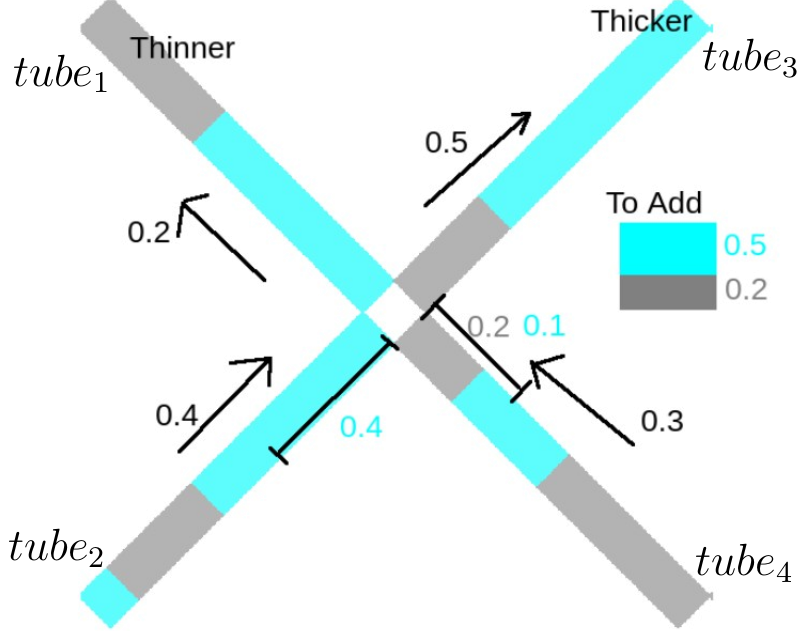
\includegraphics[width=0.45\textwidth]{fig_distributing_phases_initial}
		\caption{Distribution prediction of different fluids in a node.}
		\label{fig:distributing_phases_initial}
	\end{figure}
	
	In figure \ref{fig:distributing_phases_initial}, fluid flows from ${tube}_2$ and ${tube}_4$ into ${tube}_1$ and ${tube}_3$. 

	From the calculation of flow rates, we determined that $0.7 u.$ (unit volumes) of fluid enters the node, while $0.7 u.$ exits the node. They must be equal due to Kirchhoff's law at the node. The total inflow of $0.7 u.$ consists of $0.4 u.$ from ${tube}_2$ and $0.3 u.$ from ${tube}_4$. The outflow consists of $0.2 u.$ into ${tube}_1$, and $0.5 u.$ into ${tube}_3$.
	
	Step-1, we calculate the sum of volume of each type of fluid flowing into the node. Here, ${tube}_2$ provides $0.4 u.$ of cyan fluid, while ${tube}_4$ provides $0.1 u.$ of cyan fluid and $0.2 u.$ of gray fluid. Summing we obtain $0.5 u.$ of cyan fluid and $0.2 u.$ of gray fluid, which needs to be distributed to the outflow tubes.
	
	\begin{figure}[H]
		\centering
		\begin{subfigure}{0.48\textwidth}
			\centering
			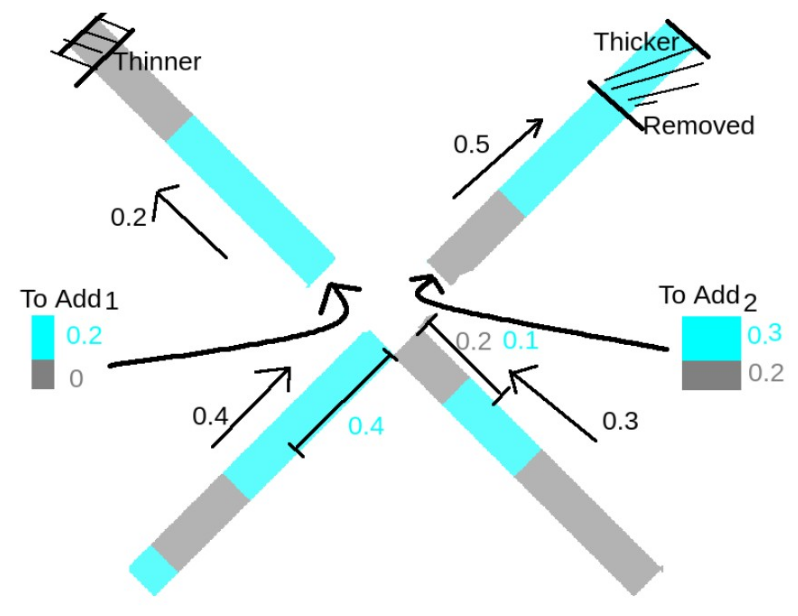
\includegraphics[width=\textwidth]{fig_distributing_phases_intermediary}
			\caption{Adding wetting phase to the thinner tube first.}
		\end{subfigure}
		\begin{subfigure}{0.42\textwidth}
			\centering
			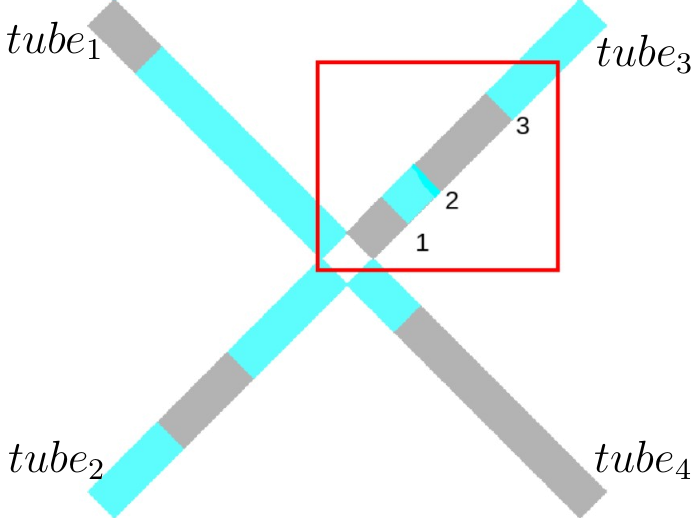
\includegraphics[width=\textwidth]{fig_distributing_phases_final}
			\caption{Final tube configuration with 3 menisci.}
			\label{fig:distributing_phases_final}
		\end{subfigure}
		\caption{Occurrence of more than 2 menisci.}
	\end{figure}
	
	Step-2, we allocate this $0.5 u.$ of cyan fluid first into the thinner tube. The thinner ${tube}_1$ takes in $0.2 u.$. This allocation space is entirely filled by $0.2 u.$ of cyan fluid. Then for the thicker tube, we need to insert $0.5 u.$ of fluid into it. $0.3 u.$ of cyan fluid is inserted first then $0.2 u.$ of gray fluid.
	
	In figure \ref{fig:distributing_phases_final}, ${tube}_1$ retains the only meniscus because the end connected to the node initially contained cyan fluid, and we introduced $0.2 u.$ of more cyan fluid. The single meniscus was just displaced upwards.
	
	However, in ${tube}_3$, gray fluid was on the end of the tube connected to the node. We added $0.3 u.$ of cyan and $0.2 u.$ of gray fluid. Since the cyan fluid entered the thicker tube first, we end up with 3 menisci.	

\subsection{Recombination} \label{sec:recombination-details}
	Our data structure was constrained to only allow the case for a maximum of two menisci in a tube. However, we see that in figure \ref{fig:distributing_phases_final} that there is possibility of more than 2 menisci occurring after distribution. We show the cases of distributing fluid in the nodes, which results in more than 2 menisci.
	
	\begin{figure}[H]
		\centering
		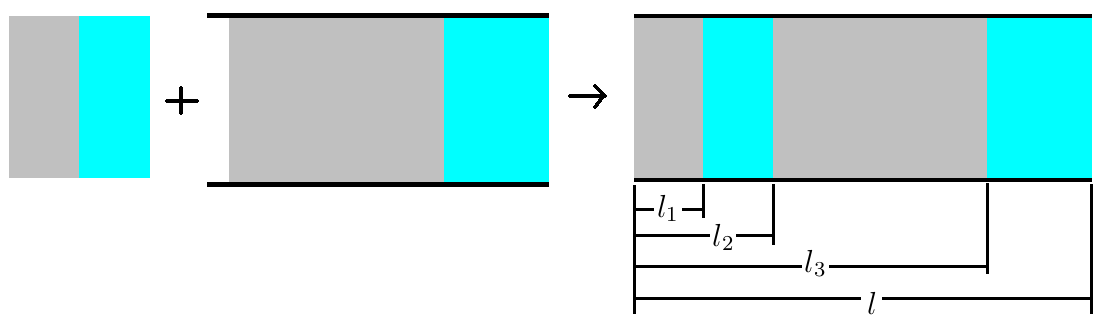
\includegraphics[width=0.8\textwidth]{fig_center-of-mass_1}
		\caption{Recombination of 3 menisci}
		\label{fig_center-of-mass_1}
	\end{figure}
	
	In figure \ref{fig_center-of-mass_1} we have a known amount of cyan and gray fluid which we need to insert into the tube. The tube which already consists of both the fluids. The flow is from left to right, so we insert the incoming fluids on the left end of the tube. Note that a block of cyan fluid always ends up in the center as it enters the tube first.
	
	Let $l_{i}$ denote the location of a meniscus. Since the tube is cylinder, the mass is simply proportional to the length they occupy in the tube, they are given by:
	
	\begin{equation}
		m_1 = l_2 - l_1 
	\end{equation}
	
	\begin{equation}
		m_2 = l - l_3
	\end{equation}
	
	Their respective center of masses $d_1$ and $d_2$ are given by:
	
	\begin{equation}	
		d_1 = \frac{l_1 + l_2}{2}
	\end{equation}
	
	\begin{equation}	
		d_2 = \frac{(l_3 + l)}{2}
	\end{equation}
	
	The center of mass of the cyan fluid in the tube is then given by:
	\begin{equation}
		d = \frac{m_1 d_1 + m_2 d_2}{m}
	\end{equation}
	
	Here,
	\begin{equation}
		m = m_1 + m_2
	\end{equation}
	
	
	We do not change the proportion of fluids in a tube during recombination. Therefore, it can be shown that if we recombine the fluids in a tube such that the center of mass of one of the fluid remained the same, then the center of mass of the other fluid will also remain the same.
	
	\begin{figure}[H]
		\centering
		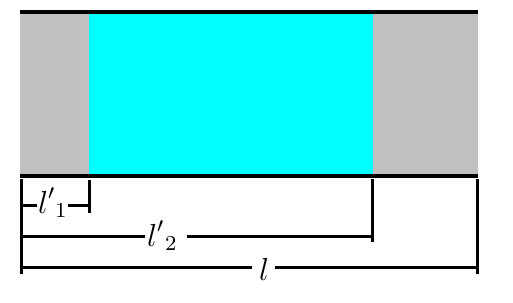
\includegraphics[width=0.4\textwidth]{fig_center-of-mass_final}
		\caption{After recombination, we always have 2 menisci}
	\end{figure}
	
	Let ${l'}_i$ denote the position of meniscus after recombination.
	
	\begin{equation}
		{l'}_1 = d - \frac{m}{2}
	\end{equation}
	
	\begin{equation}
		{l'}_2 = d + \frac{m}{2}
	\end{equation}
	

	\begin{figure}[H]
		\centering
		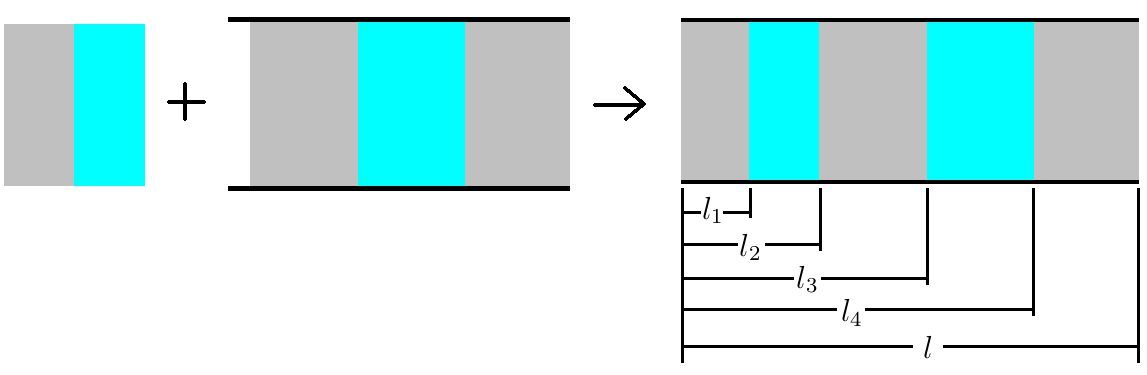
\includegraphics[width=0.9\textwidth]{fig_center-of-mass_2}
		\caption{Recombination of 4 menisci}
	\end{figure}
	
	When there are 4 menisci, we repeat the same process, except here:
	\begin{equation}
		m_2 = l_4 - l_3
	\end{equation}
	
	And
	
	\begin{equation}	
		d_2 = \frac{(l_3 + l_4)}{2}
	\end{equation}

\subsection{Flow rate in a tube with one meniscus} \label{sec:simple-flow-rate}
	At first we derive the equation for flow rate when there is one meniscus present in a tube, then we generalize the case for $n$ menisci. The flow rate of a viscous fluid through a thin tube is given by the Hagen–Poiseuille equation:
	
	\begin{equation} \label{eq:flow-rate}
		Q = \frac{\pi}{8\mu} \frac{\Delta P}{l} R^4
	\end{equation}
	
	Here, $Q$ is the volumetric flow rate in $[m^3/s]$, $\Delta P$ is the pressure difference between the ends of the tube, $\mu$ is the viscosity in $[kg/m.s]$, $l$ is the length of the tube, $R$ is the radius of the tube.
	
	\begin{figure}[H]
		\centering
		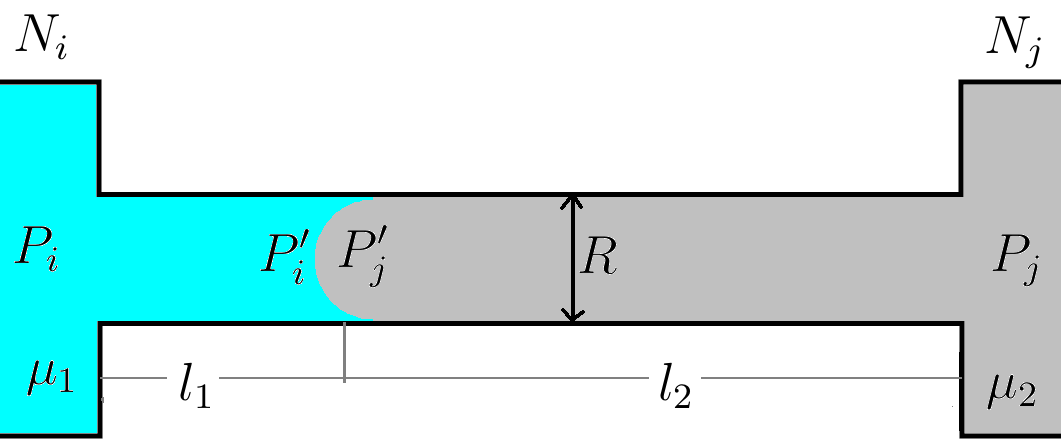
\includegraphics[height=3cm]{fig_capillary_pressure_in_tube_1mns_blue}
		\caption{Orientation of the meniscus, the convex side contains wetting fluid while the concave side contains non-wetting fluid.}
		\label{fig_capillary_pressure_in_tube_1mns_blue}
	\end{figure}
	
	In figure \ref{fig_capillary_pressure_in_tube_1mns_blue}, node $N_{i}$ kept at a pressure of $P_{i}$, and is filled with a wetting fluid of viscosity $\mu_{1}$. Node $N_{j}$ kept at a pressure of $P_{j}$ is filled with a non-wetting fluid of viscosity $\mu_{2}$. It is evident that the pressure on the convex size or on the part of the wetting fluid is lower.
	
	\begin{equation}
		P_{i}' < P_{j}'
	\end{equation}
	
	The pressure jump is given by:
	
	\begin{equation} \label{eq:capillary_pressure_mns}
		P_{j}' - P_{i}' = \frac{2 \sigma}{R}
	\end{equation}
	
	Here, $\sigma$ is the coefficient of surface tension in $[Pa.m]$ or $[kg/s]$.
	
	Separating figure \ref{fig_capillary_pressure_in_tube_1mns_blue} into two tubes of lengths $l_{1}$ and $l_{2}$, containing fluids of viscosity ${\mu}_1$ and ${\mu}_2$. The flow rates of the tubes, from equation \ref{eq:flow-rate} are given by:
	
	\begin{equation} \label{eq:flow-rate-first}
		Q = \frac{\pi}{8{\mu}_1} \frac{P_i - P^{'}_i}{l_1} R^4
	\end{equation}
	
	\begin{equation} \label{eq:flow-rate-second}
		Q = \frac{\pi}{8{\mu}_2} \frac{P^{'}_j - P_j}{l_2} R^4
	\end{equation}
	
	Due to the law of conservation of volume, the flow rates are equal. Adding the equations \ref{eq:flow-rate-first} and \label{eq:flow-rate-second}:
	
	\begin{equation} \label{eq:flow-rate-intermediate}
		Q({\mu}_1 l_1 + {\mu}_2 l_2) = \frac{\pi}{8}R^4(P_i - P_j + P^{'}_j - P^{'}_i)
	\end{equation}
	
	Substituting the equation \ref{eq:capillary_pressure_mns} about capillary pressure,
	\begin{equation} \label{eq:flow-rate-1mns-basic-m}
		Q = \frac{\pi R^4}{8Ml} \left( \Delta P_{ij} + \frac{2\sigma}{R} \right)
	\end{equation}
	
	Here,
	\begin{equation} \label{eq:def-pressure-difference} 
		\Delta P_{ij} = P_{i} - P_{j}
	\end{equation}
	
	And $M$ is the viscosity parameter:
	\begin{equation}
		M = \sum_{k} \mu_{k} \frac{l_{k}}{l}
	\end{equation}
	Note that the viscosity parameter, remains the same for any number of menisci present in a tube.
	
\subsection{Flow rate in a tube with multiple menisci} \label{sec:multi-menisci-flow-rate}
	\begin{figure}[H]
		\centering
		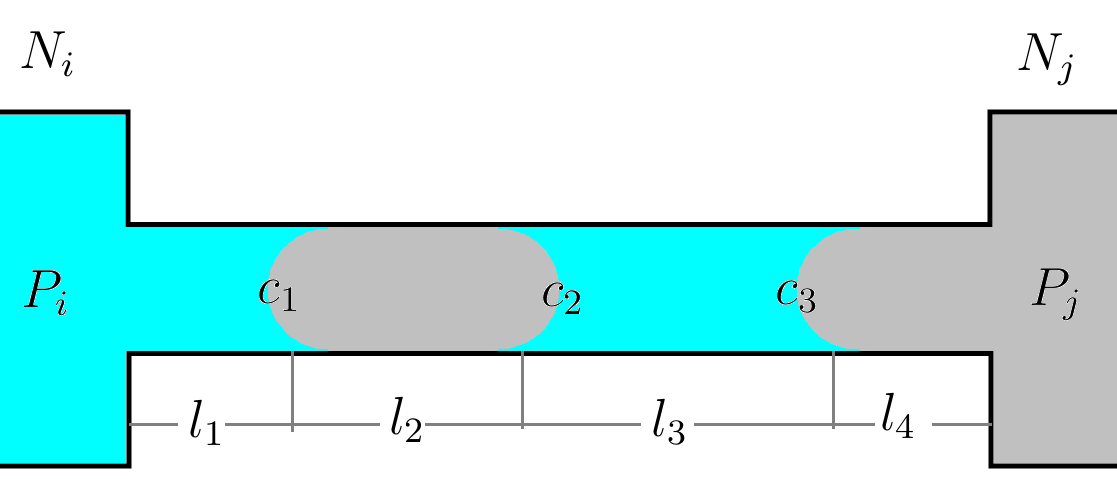
\includegraphics[height=3cm]{fig_capillary_pressure_in_tube_3mns}
		\caption{Capillary pressure contribution, $s = 1$}
		\label{fig:capillary_pressure_in_tube_3mns}
	\end{figure}
	
	Let the capillary pressures be denoted by the following:
	\begin{equation}
		c_1 = -c_2 = c_3 = \frac{2 \sigma}{R}
	\end{equation}
	
	Then for figure \ref{fig:capillary_pressure_in_tube_3mns}, the flow rate is given by:
	
	\begin{equation}
		Q = \frac{\pi R^4}{8Ml} \left( \Delta P_{ij} + c_1 + c_2 + c_3 \right)
	\end{equation}
	
	\begin{equation}
		Q = \frac{\pi R^4}{8Ml} \left( \Delta P_{ij} + \sum_{k} c_{k} \right)
	\end{equation}
	
	Flow rate for an arbitrary number of meniscus for a cylindrical tube, is given by:
	
	\begin{equation} \label{eq:main-flow-rate-with-s}
		\boxed{Q = \frac{\pi R^4}{8Ml} \left( \Delta P_{ij} + \frac{2s \sigma}{R} \right)}
	\end{equation}
	
	Where,
	
	\begin{equation} \label{eq:sign-func-def}
		s(d, n_{mns}) = 
		\begin{dcases}
			-1,&\text{$n_{mns}$ = 1, $d$ points away from $N_{i}$}\\
			0,&\text{$n_{mns}$ = 0, 2}\\
			+1,&\text{$n_{mns}$ = 1, $d$ points towards $N_{i}$}
		\end{dcases}
	\end{equation}
	
	Here,
	\begin{itemize}
		\item $d$, the direction the convex side of the meniscus points towards
		\item $n_{mns}$, the number of meniscus in a tube
	\end{itemize}
	
	In our model, the data structure does not accommodate more than 2 meniscus in a tube, hence in the definition of $s$, $n_{mns} \le 2$. Shown that, for figure \ref{fig:capillary_pressure_in_tube_3mns}, \ref{fig:capillary_pressure_in_tube_1mns_grey}, and \ref{fig:capillary_pressure_in_tube_2mns}, $s$ is $1$, $-1$, and $0$ respectively.
	
	\begin{figure}[H]
		\centering
		\begin{subfigure}{0.45\textwidth}
			\centering
			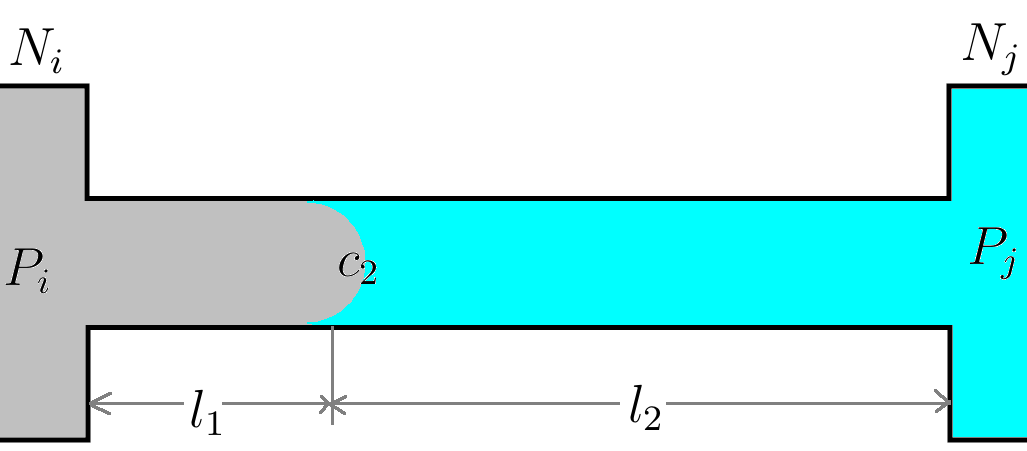
\includegraphics[width=\textwidth]{fig_capillary_pressure_in_tube_1mns_grey}
			\caption{$s = -1$}
			\label{fig:capillary_pressure_in_tube_1mns_grey}
		\end{subfigure}
		\hfill
		\begin{subfigure}{0.48\textwidth}
			\centering
			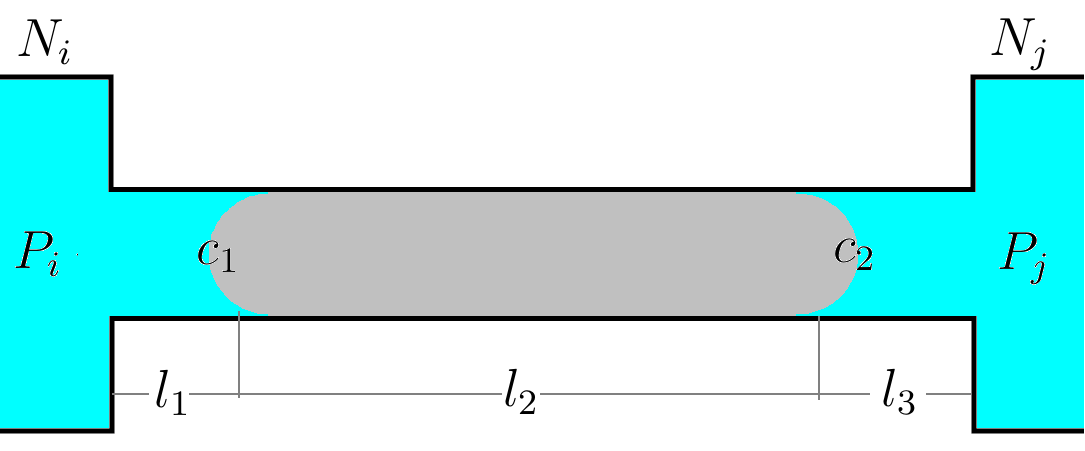
\includegraphics[width=\textwidth]{fig_capillary_pressure_in_tube_2mns}
			\caption{$s = 0$}
			\label{fig:capillary_pressure_in_tube_2mns}
		\end{subfigure}
		\caption{Capillary pressure contribution.}
	\end{figure}
		
	
\subsection{Flow rate and velocity} \label{sec:flow-rate-vel}
	Therefore, in equation \ref{eq:flow-rate-simple-coeff}, we get:
	
	\begin{equation} \label{eq:flow-rate-aij}
		A_{ij} = \frac{\pi R_{ij}^4}{8M_{ij}l} \Delta P_{ij}
	\end{equation}
	
	\begin{equation} \label{eq:flow-rate-bij}
		B_{ij} = \frac{\pi R_{ij}^4}{8M_{ij}l} \frac{2 s_{ij} \sigma}{R_{ij}}
	\end{equation}
	
	Here, note that:
	\begin{equation}
		R_{ij} = R_{ji}
	\end{equation}
	
	\begin{equation}
		M_{ij} = M_{ji}
	\end{equation}
	
	\begin{equation}
		P_{ij} = -P_{ji}
	\end{equation}
	
	\begin{equation}
		s_{ij} = -s_{ji}
	\end{equation}
	
	It clear that:
	\begin{equation} \label{eq:symmetry-of-a}
		A_{ij} = A_{ji}
	\end{equation}
	
	\begin{equation} \label{eq:symmetry-of-b}
		B_{ij} = -B_{ji}
	\end{equation}
	
	When the pressures are known in each nodes, the velocity is determined by:
	\begin{equation} \label{eq:velocity-from-pressures}
		v_{ij} = \frac{Q_{ij}}{\pi R_{ij}^2} = \frac{R_{ij}^2}{8M_{ij}l} \left( \Delta P_{ij} + \frac{2s_{ij} \sigma}{R_{ij}} \right)
	\end{equation}
